\documentclass[9pt,twocolumn,twoside]{styles/osajnl}
\usepackage{fancyvrb}
\usepackage{hyperref}
\journal{i524} 

\title{Robot Operating System (ROS): A Useful Overview}

\author[1]{Matthew Lawson}

\affil[1]{School of Informatics and Computing, Bloomington, IN 47408, U.S.A.}

\affil[*]{Corresponding authors: laszewski@gmail.com}

\dates{paper2, \today}

\ociscodes{Cloud, I524, robot, ros, ROS}

% replace this with your url in github/gitlab
\doi{\url{https://github.com/eunosm3/classes/blob/master/docs/source/format/report/report.pdf}}


\begin{abstract}
placeholder text
\newline
\end{abstract}

\setboolean{displaycopyright}{true}

\begin{document}

\maketitle

\section{Introduction}

\section{Examples of Article Components}
\label{sec:examples}

The sections below show examples of different article components.

\section{Figures and Tables}

It is not necessary to place figures and tables at the back of the
manuscript. Figures and tables should be sized as they are to appear
in the final article. Do not include a separate list of figure
captions and table titles.

Figures and Tables should be labelled and referenced in the standard
way using the \verb|\label{}| and \verb|\ref{}| commands.

\subsection{Sample Figure}

Figure \ref{fig:false-color} shows an example figure.

\begin{figure}[htbp]
\centering
\fbox{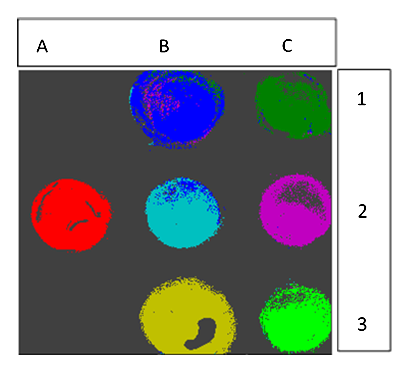
\includegraphics[width=\linewidth]{images/sample}}
\caption{False-color image, where each pixel is assigned to one of seven reference spectra.}
\label{fig:false-color}
\end{figure}

\subsection{Sample Table}

Table \ref{tab:shape-functions} shows an example table.

\begin{table}[htbp]
\centering
\caption{\bf Shape Functions for Quadratic Line Elements}
\begin{tabular}{ccc}
\hline
local node & $\{N\}_m$ & $\{\Phi_i\}_m$ $(i=x,y,z)$ \\
\hline
$m = 1$ & $L_1(2L_1-1)$ & $\Phi_{i1}$ \\
$m = 2$ & $L_2(2L_2-1)$ & $\Phi_{i2}$ \\
$m = 3$ & $L_3=4L_1L_2$ & $\Phi_{i3}$ \\
\hline
\end{tabular}
  \label{tab:shape-functions}
\end{table}

\section{Sample Equation}

Let $X_1, X_2, \ldots, X_n$ be a sequence of independent and
identically distributed random variables with $\text{E}[X_i] = \mu$
and $\text{Var}[X_i] = \sigma^2 < \infty$, and let

\begin{equation}
S_n = \frac{X_1 + X_2 + \cdots + X_n}{n}
      = \frac{1}{n}\sum_{i}^{n} X_i
\label{eq:refname1}
\end{equation}

denote their mean. Then as $n$ approaches infinity, the random
variables $\sqrt{n}(S_n - \mu)$ converge in distribution to a normal
$\mathcal{N}(0, \sigma^2)$. 

\section{Sample Algorithm}

Algorithms can be included using the commands as shown in algorithm
\ref{alg:euclid}.

\begin{algorithm}
\caption{Euclid’s algorithm}\label{alg:euclid}
\begin{algorithmic}[1]
\Procedure{Euclid}{$a,b$}\Comment{The g.c.d. of a and b}
\State $r\gets a\bmod b$
\While{$r\not=0$}\Comment{We have the answer if r is 0}
\State $a\gets b$
\State $b\gets r$
\State $r\gets a\bmod b$
\EndWhile\label{euclidendwhile}
\State \textbf{return} $b$\Comment{The gcd is b}
\EndProcedure
\end{algorithmic}
\end{algorithm}

\begin{algorithm}
\caption{Python example}\label{alg:python}
\begin{quote}
\begin{Verbatim}[numbers=left]
for i in range(0,100):
  print i
\end{Verbatim}
\end{quote}
\end{algorithm}

\section{Reference Management}

The best programs to manage your references is jabref or emacs. You
can edit the references and verify them with them for format
errors. To cite them use the citation key. You can add multiple bib
files to the bibliography command separated by comma.

\noindent Add citations with the cite command. See
\cite{las14cloudmeshmultiple} for an example on how to use multiple
clouds. In \cite{www-i524} we list the class content.

Here a test of a citation with an underscore in the url \cite{www-underscore}.

\section*{Acknowledgements}

Funding information should be listed in this section. Please evaluate
if you like to list your employer that may have funded your activities
here.  If you receive grants or project numbers, as shown in the
example.  This work was in part supported by National Science
Foundation (NSF) (1234567, 891012345) (These numbers are invented)

The acknowledgments may also contain any information that is not
related to funding:

The authors thank H. Haase, C. Wiede, and J. Gabler for technical
support.


% Bibliography

\bibliography{references}
 
\section*{Author Biographies}
\begingroup
\setlength\intextsep{0pt}
\begin{minipage}[t][3.2cm][t]{1.0\columnwidth} % Adjust height [3.2cm] as required for separation of bio photos.
  \begin{wrapfigure}{L}{0.25\columnwidth}
    
\includegraphics[width=0.25\columnwidth]{images/john_smith.eps}
  \end{wrapfigure}
  \noindent
  {\bfseries John Smith} received his BSc (Mathematics) in 2000 from
  The University of Maryland. His research interests include lasers
  and optics. 
\end{minipage}
\begin{minipage}[t][3.2cm][t]{1.0\columnwidth} % Adjust height [3.2cm] as required for separation of bio photos.
  \begin{wrapfigure}{L}{0.25\columnwidth}
    
\includegraphics[width=0.25\columnwidth]{images/alice_smith.eps}
  \end{wrapfigure}
  \noindent
  {\bfseries Alice Smith} received her BSc (Mathematics) in 2000 from
  The University of Maryland. Her research interests also include
  lasers and optics. 
\end{minipage}
\begin{minipage}[t][3.2cm][t]{1.0\columnwidth} % Adjust height [3.2cm] as required for separation of bio photos.
  \begin{wrapfigure}{L}{0.25\columnwidth}
    
\includegraphics[width=0.25\columnwidth]{images/alice_smith.eps}
  \end{wrapfigure}
  \noindent
  {\bfseries Bruce Wayne} received his BSc (Aeronautics) in 2000 from
  Indiana University. His research interests include lasers and optics.
\end{minipage}
\endgroup

\newpage

\appendix

\section{Work Breakdown}

The work on this project was distributed as follows between the
authors:

\begin{description}

\item[Matthew Lawson.] Matthew researched and wrote all of the material for this paper.

\end{description}

\section{Report Checklist}

\begin{itemize}
\renewcommand{\labelitemi}{\scriptsize$\square$} 
\item Have you written the report in word or LaTeX in the specified
  format?
\item Have you included the report in github/lab?
\item Have you specified the names and e-mails of all team members in
  your report. E.g. the username in Canvas?
\item Have you included the HID of all team members?
\item Does the report have the project number added to it?
\item Have you included all images in native and PDF format in gitlab
  in the images folder?
\item Have you added the bibliography file in bibtex format?
\item Have you submitted an additional page that describes who did
  what in the project or report?
\item Have you spellchecked the paper?
\item Have you made sure you do not plagiarize?
\item Have you made sure that the important directories are all lower
  case and have no underscore or space in it?
\item Have you made sure that all authors have a README.rst in their
  HID github/lab repository?
\item Have you made sure that there is a README.rst in the project
  directory and that it is properly filled out?
\item Have you put a work breakdown in the document if you worked in a
  group?
\end{itemize}

\section{Possible technology paper outline}

The next sections are just some suggestions, your may want to add
sections and subsections as you see fit. Images and references do not
count towards the 2 page length. Please use the \verb|\section|,
\verb|\subsection|, and \verb|\subsubsection| commands in your
paper. do not introduce hardcoded numbers. Use the \verb|\ref| and
\verb|\label| commands to refer
 to the sections.


\paragraph{Abstract}

01) ROS provides an OS for robots.  It runs exclusively on linux; Ubuntu is suggested <<- add citation
02) The main components consist of a) the pubsub communication system, b) something else and c) some final thing.
03) Roboticists and other users can interact w/ ROS via the following methods: a) C++ programs, b) ROS on linux, c) etc.
04) ROS offers a two different GUIs as well as a CLI with an extensve library of command-line tools.  Gazebo offers a CLI and a GUI, but the GUI only exists as part of the simulation process.
05) The Open Source Robotics Foundation, hereinafter OSRF, distributes ROS under some free license, probably a variant of GPL.
06) Since ROS dominates the robot software market, it has a vast ecosystem of compatible software and hardware.
07) Researchers and robot industry participants use ROS extensively.  For instance, a) foo; b) bar; and c) foobar.  Big data uses remain limited.
08) Explore ROS more by visiting \url{www.ros.org}.

\begin{figure*}[htbp]
\centering
\fbox{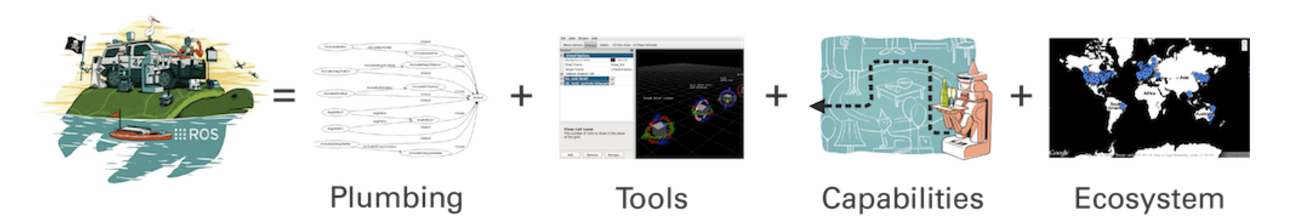
\includegraphics[width=\linewidth]{images/rosOverview.png}}
\caption{The Main Elements of ROS - the \textit{R}obot \textit{O}perating \textit{S}ystem \cite{www-ros-about}}
\label{fig:rosOverview}
\end{figure*}

\paragraph{1. Introduction}

The aptly-named \textit{Robot Operating System}, or ROS, provides a framework for writing operating systems for robots.  ROS offers "a collection of tools, libraries, and conventions [meant to] simplify the task of creating complex and robust robot behavior across a wide variety of robotic platforms" \cite{www-rosmain}. ROS' designers, the Open Source Robotics Foundation, hereinafter OSRF or the Foundation, attempt to meet the aforementioned objective by implementing ROS as a modular system.  That is, ROS offers a core set of features, such as inter-process communication, that work with or without pre-existing, self-contained components for other tasks.

\paragraph{2. Architecture} 

The OSRF designed ROS as a distributed, modular system.  The OSRF maintains a subset of essential features for ROS, i.e., \textit{ROS core}, to provide an extensible platform for other roboticists.  The Foundation also coordinates the maintenance and distribution of a vast array of ROS add-ons, referred to as modules.  ROS' core consists of the following components: a) communications infrastructure; b) robot-specific features; and, c)tools.  The modules, analagous to packages in Linux repositories or libraries in other software packages such as \textit{R}, provide solutions for numerous robot-related problems.  General categories include a) 

\subparagraph{Communications Infrastructure}
ROS implements a publish-subscribe, hereinafter pubsub, inter-process communication method as its most-basic solution for roboticists.  


\subparagraph{Robot-Specific Features}

\subparagraph{Tools}

% "If applicable include a description about architectural details. This may include a figure. Make sure that if you copy a figure you put the \cite{?} in the caption also. Otherwise it is plagiarism."

\paragraph{2.1. API}

comment on the API which could include language bindings

\paragraph{2.2. Shell Access}

If applicable comment on how the tool can be used from the command line

\paragraph{2.3.Graphical Interface}

ROS includes two GUIs, \textit{rviz} and \textit{rqt} \cite{www-ros-core-components}.  rviz creates 3D visualizations of the robot, as well as the sensors and sensor data specified by the user.  This component renders the robot in 3D based on a user-supplied description in XML format, referred to as a Unified Robot Description Format, herinafter URDF, document.  The machine-readable URDF describes all of the features of the robot, including how the components look, the size and number of wheels or the size and number of appendages and joints, the types of sensors available to the robot and the location of the sensors.

rviz also visualizes the data collected by the sensors.  For instance, it can combine camera images and laser scans to render a robot's environment, actual or virtual, from the robot's perspective.  

rqt utilizes allows users to create graphical interfaces for various aspects of the robot via a \textit{Qt}-based system \cite{www-wiki-qt}.



\paragraph{3. Licensing}

The Open Source Robotics Foundation, hereinafter OSRF, distributes the core of ROS under the standard, three-clause BSD license, hereinafter BSD-3 license.  The BSD-3 license belongs to a broader class of copyright licenses referred to as \textit{permissive licenses} because it imposes zero restrictions on the software's redistribution as long as the redistribution maintains the license's copyright notices and warranty disclaimers \cite{www-wikipedia-bsd}.

Other names for BSD-3 include: a) BSD-new; b) New BSD; c) revised BSD; d) The BSD License, the official name used by the Open Source Initiative; and, e) Modfied BSD License, used by the Free Software Foundation.

% The core of ROS is licensed under the standard three-clause BSD license. This is a very permissive open license that allows for reuse in commercial and closed source products. You can find more about the BSD license here:

% http://opensource.org/licenses/BSD-3-Clause
% http://en.wikipedia.org/wiki/BSD_licenses
% While the core parts of ROS are licensed under the BSD license, other licenses are commonly used in the community packages, such as the Apache 2.0 license, the GPL license, the MIT license, and even proprietary licenses. Each package in the ROS ecosystem is required to specify a license, so that it is easy for you to quickly identify if a package will meet your licensing needs.\paragraph{4. Ecosystem}

ROS has more than 3,000 components available from its distributed community, including proof-of-concept algos to industrial-quality software drivers. \cite{www-ros-about}.

% Some technologies have a large ecosystem developed around them with
% extensions plugins and other useful tools. Identify if they exists and
% comment on what they can achieve

% provide potentially a mindmap or a figure illustrating how the
% technology fits in with other technologies if applicable.

\paragraph{4. Use Cases}

\paragraph{4.1. Use Cases  for Big Data}

Locate and describe major usecases that demonstrate the technology
while focussing on big data related use cases. Make sure you do proper
references with the \cite{?} command. Do not put URLs in the text.

\paragraph {4.2. Other Use Cases}

Some technologies may not just be used for big data, find other makor
use cases from other areas if applicable.  Make sure you do proper
references with the \cite{?} command. Do not put URLs in the text.

\paragraph{5. Educational material}

Put information here how someone would find out more about the
technology. Use important material and do not list hundrets of web
pages, be selective.

\paragraph{6. Conclusion}

Put in some conclusion based on what you have researched

\paragraph{Acknowledgement}

Put in the information for this class and who may sponsor
you. Examples will be given later

\end{document}
